\chapter{Проектирование системы}
\label{chapter3}

В данном разделе описывается инженерная часть научно-исследовательской работы, а именно проектирование прототипа системы генерации документов на основе шаблонов. Представлены требования к проектируемому модулю, описан выбор средств для  описания результатов проектирования. Также описывается разработка функциональной структуры информационной системы.




\section{3.1. Выбор средств (языка) для описания результатов проектирования}


В данном разделе приведен сравнительный анализ и выбор средств (языка) для описания результатов проектирования. Описаны основные достоинства и приведены обоснования сделанного выбора относительно решения конечной задачи.


В данной работе в качестве языка проектирования был выбран язык UML, так как он обладает рядом преимуществ:
\begin{enumerate}

\item Визуальная интерпретация

UML-диаграмма - это визуальное представление отношений между классами и сущностями в компьютерной программе. Класс - это объект в программировании, который организует аналогичные переменные и функции в одном месте. Чтобы понять программу, важно понять, что делает каждый объект класса, хранящаяся в нем информация и как она относится к другим классам в программе. Показывая эту информацию на диаграмме, легко понять и визуализировать отношения программы.

\item Читаемость и повторное использование

Диаграмма UML выгодна тем, что она очень читаема. Диаграмма предназначена для понимания любым программистом и помогает объяснить отношения в программе простым способом. Традиционно, чтобы понять программу, программист будет читать код напрямую. Это может быть тысячи или миллионы строк кода в очень больших программах. Наличие UML-диаграммы помогает быстро проиллюстрировать эти отношения. Кроме того, используя диаграмму для отображения кода, запущенного в программе, программист может видеть избыточный код и повторно использовать части кода, которые уже существуют, а не переписывать эти функции.

\item Стандарт

UML - это текущий стандарт программирования в объектно-ориентированных языках программирования. При создании классов и других объектов с отношениями между собой UML используется для визуального описания этих отношений. Поскольку он используется в качестве стандарта, он широко понимается и хорошо известен. Это позволяет новому программисту вступить в проект и быть продуктивным с первого дня.

\end{enumerate}
\cite{nou}
UML - унифицированный язык моделирования. Из этих трех слов главным является слово " язык ".

    Язык - это система знаков, служащая:
\begin{enumerate}


        \item средством человеческого общения и мыслительной деятельности;
        \item способом выражения самосознания личности;
        \item средством хранения и передачи информации.
\end{enumerate}
\cite{craig_uml}
    Язык включает в себя набор знаков (словарь) и правила их употребления и интерпретации (грамматику).

Актуальность построения диаграмм объясняется тем, что разработка модели любой системы (не только программной) всегда предшествует ее созданию или обновлению. Это необходимо хотя бы для того, чтобы яснее представить себе решаемую задачу. Продуманные модели очень важны и для взаимодействия внутри команды разработчиков, и для взаимопонимания с заказчиком. В конце концов, это позволяет убедиться в "архитектурной согласованности" проекта до того, как он будет реализован в коде.



\section{3.2. Проектирование системы программных веб-интерфейсов}


В данном разделе описан процесс и представлены результаты проектирования системы программных веб-интерфейсов для разрабатываемого прототипа.


Для проектирования архитектуры модуля был использован объектно- ориентированный подход.
Объектно-ориентированное программирование рассматривает абстрактные сущности, называемые объектами. Эти сущности могут пониматься как совокупность выделенных свойств. Опираясь на них и отношения между ними, мы можем реализовывать сложную логику приложения. 

Программный модуль, разрабатываемый в данной работе состоит пакетов и классов, составляющих само приложение. Основные пакеты следующие: EasyDox, EasyDox.Morpher, Microsoft.Office.Interop.Excel, Microsoft.Office.Interop.Word. Первые два пакета необходимы для заполнения шаблона документа данными и склонения определенных словесных конструкций, таких как ФИО, по падежам. Последние два пакета включают в себя функции, упрощающие доступ к объектам API Office. Основными классами являются DataImport, Declination, DataExport.

DataImport отвечает за чтение файла базы данных посредством методов пакета Interop и извлечения необходимых данных. Также , для импорта данных использовалась пользовательская библиотека EasyDox, в которой прописан класс Engine, отвечающий за заполнение шаблонов данными.

Declination отвечает за склонение необходимых словесных конструкций по падежам. Для этого используется библиотека EasyDox.Morpher параметры которой передаются в конструктор класса Engine.
 
DataExport отвечает за генерирование нового документа Word, с полями шаблона, заполненными необходимой информацией изучаемой предметной области.
В результате проектирования программного модуля была получена диаграмма классов, представленная на рисунке 3.1.

\begin{figure}
	\caption{Диаграмма классов}
	\centering
	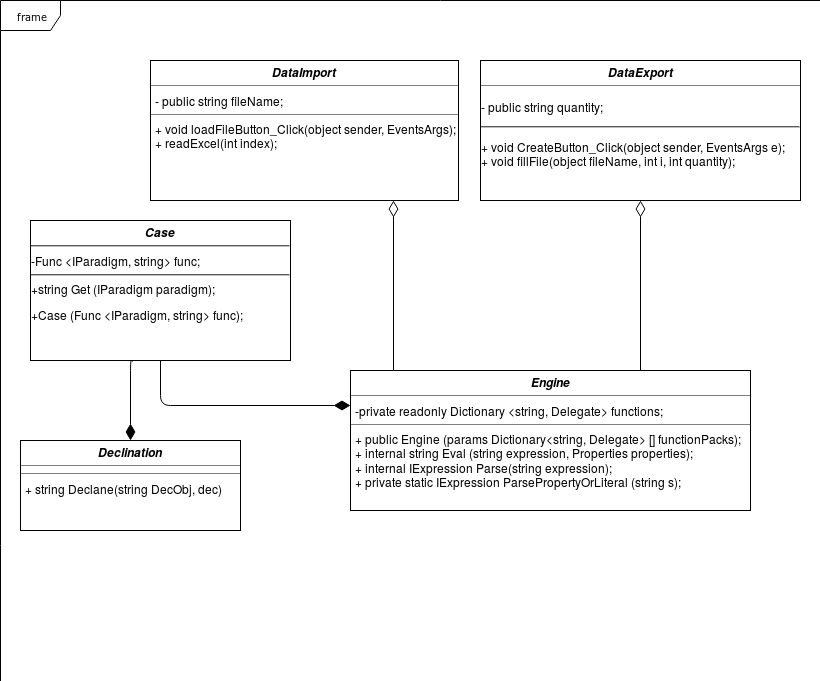
\includegraphics[width=\textwidth]{./UIR Class.png}
\end{figure}

\section{3.3. Разработка функциональной структуры информационной системы}

В данном разделе описывается процесс разработки функциональной структуры информационной системы. Описаны основные функции и связи.


Одним из основных методов является метод класса DataImport - ReadExcel, который позволяет при помощи встроенных методов пакета Interop взаимодействовать с объектами Excel, а конкретно получать необходимые файлы из ячеек базы данных. 
Метод ReadTemplate класса DataExport позволяет открыть заданный шаблон и найти в нем поля для заполнения необходимыми данными.
Метод Decline класса Declination склоняет словесные конструкции русского языка по заданным падежам, а метод FillData класса DataExport заполняет поля шаблона готовыми данными в необходимых падежах и создаёт новый документ (отчёт) Word. В простейшей версии пользовательского интерфейса пользователь сможет выбирать базу данных (Excel), шаблон документа (Word), а также задавать число итераций, для получения желаемого количества отчётов. При дальнейшей разработке планируется создание веб-сервиса с доработанным функционалом, а также серверным и клиентским кодом.
\cite{mcrsft}

\section{3.4. Выводы}

В данном разделе подводятся итоги проектирования разрабатываемой системы.

В данной главе описаны основные пакеты, которые содержит разрабатываемый программный
модуль, а также перечислены классы, включенные в эти пакеты. По итогам данного этапа проектирования получена архитектура системы, которая отражает ключевые моменты реализации модуля.









